\documentclass[english,onecolumn]{IEEEtran}
\usepackage[T1]{fontenc}
\usepackage[latin9]{luainputenc}
\usepackage[letterpaper]{geometry}
\geometry{verbose}
\usepackage{amsfonts}
\usepackage{babel}

\usepackage{extarrows}
\usepackage[colorlinks]{hyperref}
\usepackage{listings}
\usepackage{xcolor}


\usepackage{amsmath,graphicx}
\usepackage{subfigure} 
\usepackage{cite}
\usepackage{amsthm,amssymb,amsfonts}
\usepackage{textcomp}
\usepackage{bm}
\usepackage{booktabs}


\providecommand{\U}[1]{\protect\rule{.1in}{.1in}}
\topmargin            -18.0mm
\textheight           226.0mm
\oddsidemargin      -4.0mm
\textwidth            166.0mm
\def\baselinestretch{1.5}

\begin{document}

\begin{center}
	\textbf{SI231 - Matrix Computations, Fall 2020-21}\\
	Homework Set \#1\\
	\texttt{Prof. Yue Qiu and Prof. Ziping Zhao} 
\par\end{center}


\noindent
\rule{\linewidth}{0.4pt}
{\bf Acknowledgements:}
\begin{enumerate}
	\item Deadline: {\bf 2020-09-27 23:59:59}
	\item No handwritten is accepted. You need to use \LaTeX. (If you have difficulty in using \LaTeX, you are allowed to use \textbf{Word} for the first and the second homework to accommodate yourself.)
	\item Do use the given template.
\end{enumerate}
\rule{\linewidth}{0.4pt}


\section{Understanding rank, range space and null space}
\textbf{Problem 1}. \textcolor{blue}{(4 points $\times$ 5)}
\begin{enumerate}
	\item For matrix $\mathbf{A}\in\mathbb{R}^{m\times n}$, prove that $\mathbb{R}^n = \mathcal{N}(\mathbf{A}) \oplus \mathcal{R}(\mathbf{A}^{T})$ \footnote{Let $\mathcal{S}_1$ and $\mathcal{S}_2$ be two subspaces of $\mathbb{R}^n$, if $\mathcal{S}_1 \cap \mathcal{S}_2 = \{ \mathbf{0}\}$ and $\mathcal{S}_1 + \mathcal{S}_2 = \mathbb{R}^n$, we define the \textbf{direct sum} $\mathbb{R}^n = \mathcal{S}_1 \oplus \mathcal{S}_2.$}.
	
	\textbf{Hint:} ${\sf dim}(\mathcal{N}(\mathbf{A})) + {\sf dim}(\mathcal{R}(\mathbf{A}^T)) = n\,.$
	
	\item For matrices $\mathbf{A}\in\mathbb{R}^{m\times n}, \mathbf{B}\in\mathbb{R}^{m\times n}$, prove that $ {\sf rank} (\mathbf{A}+\mathbf{B})\leq {\sf rank}(\mathbf{A}) + {\sf rank}(\mathbf{B}).$ 
	
	\item For matrices $\mathbf{A}\in\mathbb{R}^{m\times n}, \mathbf{B}\in\mathbb{R}^{n\times p},$ prove that ${\sf rank} (\mathbf{A B})\leq \min\{ {\sf rank}(\mathbf{A}), {\sf rank}(\mathbf{B}) \}$ and ${\sf rank}(\mathbf{AB}) = n$ only when $\mathbf{A}$ has full-column rank and $\mathbf{B}$ has full-row rank. 
		
	\item For matrix $\mathbf{A}\in\mathbb{R}^{m\times n}$ and $\mathbf{B}\in\mathbb{R}^{m\times p}$, prove that $\mathcal{R}(\mathbf{A|B}) = \mathcal{R}(\mathbf{A}) + \mathcal{R}(\mathbf{B})$
	\footnote{Here $\mathbf{A|B}$ denotes a new matrix combined by $\mathbf{A}$ and $\mathbf{B}$. For example, $\mathbf{A} = \begin{bmatrix}
		a_{11} & a_{12} \\
		a_{21} & a_{22}
		\end{bmatrix}$, $\mathbf{B} = \begin{bmatrix}
		b_{11} \\
		b_{21}
		\end{bmatrix}$, then $\mathbf{A|B} = \begin{bmatrix}
		a_{11} & a_{12} & b_{11} \\
		a_{21} & a_{22} & b_{21}
		\end{bmatrix}$.}
	
	\item  For matrix $\mathbf{A}\in\mathbb{R}^{m\times n}$ and $\mathbf{B}\in\mathbb{R}^{m\times p}$, prove that
	\[
	{\sf rank}(\mathbf{A|B}) = {\sf rank}(\mathbf{A}) + {\sf rank}(\mathbf{B})  - \text{dim}(\mathcal{R}(\mathbf{A})\cap \mathcal{R}(\mathbf{B}))\,.
	\]
	\textbf{Hint:} Recall the result in 4). 
\end{enumerate}




\newpage
\section{Understanding span, subspace}
\noindent\textbf{Problem 1.}  \textcolor{blue}{(10 points)} 
For a set of vectors $\mathcal{S} = \{ \mathbf{v}_1, \ldots, \mathbf{v}_n\}$, prove that $\text{span}(\mathcal{S})$ is the intersection of all subspaces that contain $\mathcal{S}$, i.e.,
prove that $\text{span}(\mathcal{S})=\mathcal{M}$ where $\mathcal{M}:=\cap_{s\subseteq \mathcal{V}} \mathcal{V}$ is the intersection of all subspaces that contain $\mathcal{S}$ and $\mathcal{V}$ denotes the subspace containing $\mathcal{S}$.

\textbf{Hint:} Prove that $\text{span}(\mathcal{S})\subseteq\mathcal{M}$ and $\mathcal{M}\subseteq \text{span}(\mathcal{S})$. 




\newpage

\section{Basis, dimension and projection}
\noindent\textbf{Problem 1.} \textcolor{blue}{(2 points $\times$ 2)} 
Determine the dimension of each of the following vector spaces:
\begin{enumerate}
	\item The space of polynomials having degree $n$ or less;
	\item The space of $n\times n$ symmetric matrices.
\end{enumerate}

\noindent\textbf{Problem 2. Some Important linear transformations}
\begin{enumerate}
	\item \textbf{Rotations.} \textcolor{blue}{(6 points)}
	A rotation matrix $\mathbf{R}\in\mathbb{R}^{n\times n}$ is an orthogonal matrix ($\mathbf{R}\mathbf{R}^T=\mathbf{I}$) such that $\det({\mathbf{R}})=1$.
	\begin{itemize}
		\item According to above definition, find all rotation matrix in $\mathbb{R}^{2\times 2}$.  
		\item Geometrically, if $\mathbf{R}\in\mathbb{R}^{2\times 2}$, then $\mathbf{Rx}$ means we rotate the vector ${\bf x}\in\mathbb{R}^2$ from some angle $\theta\in[0,2\pi]$ in anti-clockwise direction. 
		For ${\bf x}=[\cos(\pi/4), \sin(\pi/4)]^T$, compute $\mathbf{Rx}$, where $\mathbf{R}$ represents the matrix that rotating ${\bf x}$ by $7/12\pi$ in anti-clockwise direction. \\
		\textbf{Hint:} draw a plot of ${\bf x}$ and $\mathbf{Rx}$.
	\end{itemize} 
	\item \textbf{Reflections.} \textcolor{blue}{(8 points)}
	 Let ${\bf u}\in\mathbb{R}^n$ be a unit vector, $ \|{\bf u}\|_2=1$. For a given vector ${\bf x}\in\mathbb{R}^n$ and a hyperplane $\mathcal{H}_u=\{ {\bf x}\in\mathbb{R}^n| {\bf u}^T{\bf x}=0\}$.
	Let $\mathbf{Q} = {\bf I}-{\bf uu}^T$.
	Then a vector ${\bf y}\in\mathbb{R}^n$ is said to be a \emph{reflection} of ${\bf x}$ with respect to $\mathcal{H}$ if their projections onto the hyperplane $\mathcal{H}$ (denoted as $\mathbf{Q}{\bf x}$ and $\mathbf{Qy}$ respectively) satisfy 
	\[
	\mathbf{Q}{\bf x}=\mathbf{Qy}\,,\quad \|{\bf x}-\mathbf{Qx}\|_2=\|{\bf y}-\mathbf{Qy}\|_2\,.
	\]
	
	See Figure.1 for visualization.
	
	\begin{figure}[h]
		\centering
		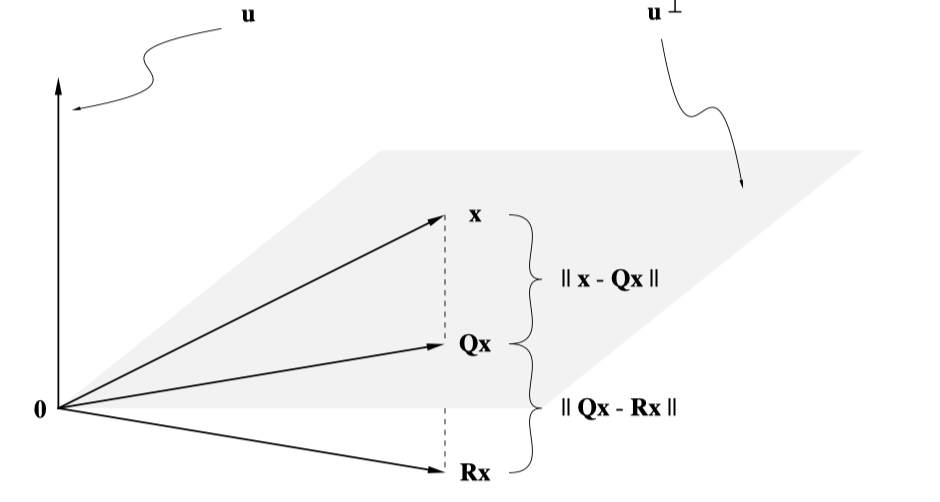
\includegraphics[width=0.5\textwidth]{reflection.png}
		\caption{Reflection of ${\bf x}$} 
	\end{figure}
	
	A Householder matrix has the form $\mathbf{H} = \mathbf{I} -2{\bf uu}^T$.
	Prove that $\mathbf{Hx}$ is a reflection of ${\bf x}$ with respect to $\mathcal{H}_u$. 
\end{enumerate}



\newpage
\section{Direct sum} 
\noindent\textbf{Problem 1.} \textcolor{blue}{(10 points)}
Let $\mathcal{V}$ be a vector space, and $\mathcal{B}$ be a basis for $\mathcal{V}$. Suppose that there exist subsets $\mathcal{B}_1, \mathcal{B}_2$ of $\mathcal{B}$, such that $\mathcal{B}=\mathcal{B}_1\cup \mathcal{B}_2$ and $\mathcal{B}_1\cap \mathcal{B}_2=\emptyset.$ Then show that $\mathcal{V}=\text{span}(\mathcal{B}_1)\oplus \text{span}(\mathcal{B}_2).$


\noindent\textbf{Problem 2.} \textcolor{blue}{(10 points)}
Let $\mathcal{V}$ be a real vector space of dimension $ n $. Let $\mathcal{S}$ be a subspace of $\mathcal{V}$ of dimension $ d \leq  n $.
Prove that there exists a subspace $\mathcal{T}$ of $\mathcal{V}$ such that $\mathcal{V}=\mathcal{S} \oplus \mathcal{T} $.



\newpage
\section{Understanding the Matrix Norm}
\noindent\textbf{Problem 1.} \textcolor{blue}{(7 points $\times$ 2)}
Matrix norm is induced by vector norm, 
\[
\|\mathbf{A}\|_p  = \max_{\mathbf{x}\ne \mathbf{0}} \frac{ \|\mathbf{Ax} \|_p}{\|\mathbf{x} \|_p} = \max_{\|\mathbf{x}\|_p= 1} \|\mathbf{Ax} \|_p\,, \quad \mathbf{A}\in \mathbb{R}^{m\times n},\mathbf{x}\in \mathbb{R}^{n\times 1}\,,
\]
prove that 
\begin{enumerate}
	\item the matrix 1-norm
	\begin{align*}
	\|\mathbf{A}\|_1  
	& =  \max_{\|\mathbf{x}\|_1= 1} \|\mathbf{Ax} \|_1 = \max_{j}\sum_{i}^m|a_{ij}|\\
	& = \text{ the largest absolute column sum.}
	\end{align*}
	\item the matrix $\infty$-norm
	\begin{align*}
	\|\mathbf{A}\|_{\infty} 
	& =  \max_{\|\mathbf{x}\|_{\infty}= 1} \|\mathbf{Ax} \|_{\infty} = \max_{i}\sum_{j}^n|a_{ij}|\\
	& = \text{ the largest absolute row sum.}
	\end{align*}
\end{enumerate} 




\newpage
\section{Understanding the H\"{o}lder inequality}
\noindent\textbf{Problem 1.} \textcolor{blue}{(6 points $\times$ 3)}
H\"{o}lder inequality:
\[
|\mathbf{x}^T\mathbf{y}| \le \|\mathbf{x}\|_p \|\mathbf{y}\|_q\,, 
\]
for any $p,q$ such that $1/p + 1/q = 1$, $p\ge 1$.
Derive this inequality by exexcuting the following steps:
\begin{enumerate}
	\item Consider the function $f(t) = (1-\lambda) + \lambda t -t^\lambda$ for $0<\lambda <1$, establish the inequality 
	\[
	\alpha^\lambda \beta^{1-\lambda}  \le \lambda \alpha +(1-\lambda)\beta\,,
	\]
	for nonnegative real numbers $\alpha$ and $\beta$.
	\item Let $\hat{\mathbf{x}} = \mathbf{x}/ \|\mathbf{x}\|_p$ and $\hat{\mathbf{y}} = \mathbf{y}/ \|\mathbf{y}|_q$, and apply the inequality of part 1) to obtain 
	\[
	\sum_{i=1}^n |\hat{x}_i \hat{y}_i| \le \frac{1}{p} \sum_{i=1}^n |\hat{x}_i|^p + \frac{1}{q} \sum_{i=1}^n |\hat{y}_i|^q = 1\,. 
	\]
	\item Deduce the H\"{o}lder inequality with the above results.
	\item \textcolor{blue}{(Bouns question: 10 points)} Prove the general form of triangle inequality 
	\[
	\| \mathbf{x} + \mathbf{y}\|_p \le \| \mathbf{x}\|_p + \|\mathbf{y}\|_p\,.
	\]
	\textbf{Hint:} For $p>1$, let $q$ be the number such that $1/q = 1- 1/p$. Verify that for scalars $\alpha$ and $\beta$,
	\[
	|\alpha + \beta|^p = |\alpha + \beta||\alpha + \beta|^{p/q} \le |\alpha||\alpha+\beta|^{p/q} + |\beta||\alpha+\beta|^{p/q}
	\]
	and make use of H\"{o}lder's inequality.
\end{enumerate}

\end{document}
